\documentclass[11pt]{article}
\usepackage[utf8]{inputenc}
\usepackage{amsmath, amssymb, mathtools}
\usepackage{geometry}
\geometry{a4paper, margin=1in}
\usepackage{graphicx}
\usepackage{caption}
\usepackage{subcaption}
\usepackage{hyperref}
\usepackage{natbib}
\usepackage{siunitx}
\sisetup{output-exponent-marker=\mathrm{e}}
\usepackage{amsfonts}
\usepackage{physics}
\usepackage{booktabs}
\usepackage{enumitem}
\usepackage{tikz}
\usepackage{pgfplots}
\pgfplotsset{compat=1.18} % Ensure compatibility with pgfplots
\usetikzlibrary{plotmarks, math}

% Font configuration (loaded last)
\usepackage{newtxtext}
\usepackage{newtxmath}

\title{Fractal Bindu ($S^3$) Reality: A Causally Interdependent Cyclic Model of the Universe}
\author{Andrei Preece \and Boris Batenin}
\date{Berlin, 2025}

\begin{document}

\maketitle

\begin{abstract}
The Universe is modeled as a compact, simply connected three-dimensional sphere ($S^3$), where Bindu---an ancient term from Advaita Vedanta embodying the indestructible essence of reality---unifies the photon and the cosmos through continuous phase transitions within a fixed topology. Mirroring the topological property of $S^3$, which remains simply connected upon removal of any point, Bindu, as a \textit{skandha}, represents a self-similar, causally interdependent process across all scales, from the Planck length ($l_P = \SI{1.616e-35}{\meter}$) to cosmological horizons. The perceived cosmic expansion, observed as redshift and growing light horizons, arises from the internal dynamics of energy density, governed by the golden ratio ($\phi = \frac{1 + \sqrt{5}}{2} \approx 1.618$), Ricci flow, and a unified wave function $\Psi_{\text{universe}}(t)$, not from a physical dilation of $S^3$. The speed of light ($c = \SI{299792458}{\meter\per\second}$) drives this unfolding, with energy fractally requantized without excess or deficiency. The $S^3$ manifold exists as the sole ontological foundation, neither eternal nor non-eternal, but causally interdependent, outside time and existence, with all phenomena arising within the observer's light sphere. Supported by cosmic microwave background (CMB) data, gravitational lensing, and quantum principles, this model offers a continuous, interconnected reality.
\end{abstract}

\section{Preamble: Ontological and Topological Foundations}
% Establishing the philosophical and topological basis
Bindu, rooted in Advaita Vedanta, is an ancient term symbolizing the indestructible, unified essence of reality, analogous to the topological structure of a three-dimensional sphere ($S^3$). Just as $S^3$ remains simply connected and equivalent to itself upon removal of any point, Bindu embodies a self-similar, causally interdependent reality that unifies all scales---from the photon to the Universe. In this model, Bindu manifests as a \textit{skandha}, a dynamic process that drives the invariant unfolding of $S^3$’s internal metric at the speed of light ($c = \SI{299792458}{\meter\per\second}$), with energy requantized fractally via the golden ratio ($\phi \approx 1.618$) across all levels of embedding, without excess or deficiency.

The $S^3$ manifold, the simplest three-dimensional manifold with a trivial fundamental group, exists as the sole ontological foundation of reality. It is neither eternal nor non-eternal, neither arising from itself, nor from another, nor from both, nor without cause, but as a causally interdependent entity outside conventional notions of time and existence. All phenomena---space, time, and cyclicity---emerge within the observer’s light sphere, defined by the invariant propagation of light. The perceived expansion, such as redshift, results from the decreasing energy density within this fixed topology, not from a physical dilation of $S^3$. This framework eliminates singularities and external boundaries, presenting a reality where all dynamics are internal, fractal, and interconnected.

\section{Bindu: The Unified Essence of Reality}
% Defining Bindu in detail
Bindu is a dynamic, homeomorphic process undergoing continuous phase transitions, unifying the photon and the Universe within the fixed topology of $S^3$. As a \textit{skandha}, it transcends locality and absolute time, acting as a self-similar node of energy and information. The internal metric of $S^3$ unfolds invariantly at the speed of light, with energy requantized fractally by $\phi$ across scales, from the Planck length ($l_P = \SI{1.616e-35}{\meter}$) to cosmological horizons.

\begin{itemize}
    \item \textbf{Photon as Bindu}: The photon is the localized expression of Bindu, a massless quantum propagating phase transitions at $c$.
    \item \textbf{Universe as Bindu}: The Universe is the spherical manifestation of Bindu, a fixed $S^3$ where energy density evolves fractally within a constant topology.
\end{itemize}

The perceived cosmic expansion arises from the observer’s light sphere, not from a physical stretching of $S^3$. Cyclicity is a perceptual effect driven by shifts in energy density within this invariant manifold.

\section{Mathematical Formalization}
% Describing the topological and mathematical framework
\subsection{Topology of $S^3$: A Fixed Manifold}
The Universe is a compact, simply connected three-dimensional sphere $S^3$ with no boundary or external embedding space. Its metric is:
\[
ds^2 = -c^2 dt^2 + R^2 d\Omega^2,
\]
where:
\begin{itemize}
    \item $c = \SI{299792458}{\meter\per\second}$,
    \item $R \approx \SI{1e26}{\meter}$ is the fixed radius of $S^3$,
    \item $d\Omega^2 = d\theta^2 + \sin^2\theta d\phi^2 + \sin^2\theta \sin^2\phi d\psi^2$.
\end{itemize}

Unlike the FLRW model with a growing scale factor $a(t)$, here $R$ is time-invariant. The perceived expansion, described as $R(t) = R_0 e^{Ht}$, is a coordinate effect due to the growth of the observer’s light sphere, driven by decreasing energy density within $S^3$.

\subsection{Unified Wave Function}
% Formalizing the wave function
The evolution of Bindu is described by:
\[
\Psi_{\text{universe}}(t) = A(t) \cdot e^{i \Theta(t)},
\]
where $A(t)$ reflects energy density, and $\Theta(t)$ encodes the internal rhythm.

\subsubsection{Amplitude $A(t)$}
\[
A(t) = \left[ A_0 \left( \frac{c t}{l_P} \right)^{-3/2} \cdot \sigma(t_{\text{rec}} - t) + B_0 e^{-\frac{3H}{2}(t - t_{\text{rec}})} \cdot \sigma(t - t_{\text{rec}}) \right],
\]
where:
\begin{itemize}
    \item $A_0 \approx \SI{1e90}{}$, normalizing to $E_{\text{total}} = \SI{7.21e69}{\joule}$,
    \item $l_P = \SI{1.616e-35}{\meter}$, $t_P = \frac{l_P}{c} = \SI{5.39e-44}{\second}$,
    \item $B_0 \approx A_0 \left( \frac{c t_{\text{rec}}}{l_P} \right)^{-3/2}$,
    \item $H = \SI{2.45e-17}{\per\second}$,
    \item $\sigma(x) = \frac{1}{1 + e^{-kx}}$, $k = \SI{1e12}{\per\second}$, $t_{\text{rec}} = \SI{1.2e13}{\second}$.
\end{itemize}

Behavior:
\begin{itemize}
    \item For $t \ll t_{\text{rec}}$: $A(t) \approx A_0 \left( \frac{c t}{l_P} \right)^{-3/2}$.
    \item For $t \gg t_{\text{rec}}$: $A(t) \approx B_0 e^{-\frac{3H}{2}(t - t_{\text{rec}})}$.
    \item At $t = t_{\text{rec}}$: Smooth crossover at $\sigma(0) = 0.5$.
\end{itemize}

\subsubsection{Phase $\Theta(t)$}
\[
\Theta(t) = \left( \frac{\phi t}{t_P} \cdot \sigma(t_{\text{rec}} - t) + H t \cdot \sigma(t - t_{\text{rec}}) \right),
\]
where $\phi \approx 1.618$. Behavior:
\begin{itemize}
    \item For $t < t_{\text{rec}}$: $\Theta(t) \approx \frac{\phi t}{t_P}$.
    \item For $t > t_{\text{rec}}$: $\Theta(t) \approx H t$.
\end{itemize}

\subsubsection{Full Expression}
\[
\Psi_{\text{universe}}(t) = \left[ A_0 \left( \frac{c t}{l_P} \right)^{-3/2} \cdot \sigma(t_{\text{rec}} - t) + B_0 e^{-\frac{3H}{2}(t - t_{\text{rec}})} \cdot \sigma(t - t_{\text{rec}}) \right] \cdot e^{i \left( \frac{\phi t}{t_P} \cdot \sigma(t_{\text{rec}} - t) + H t \cdot \sigma(t - t_{\text{rec}}) \right)}.
\]
Normalization: $\abs{\Psi_{\text{universe}}(t)}^2 \propto \rho(t)$, with $\rho(t) = \frac{E_{\text{total}}}{\frac{4}{3} \pi (R_0 e^{Ht})^3}$.

\subsection{Fractal Energy Distribution}
% Describing fractal scaling
Energy density scales fractally:
\[
\rho_n = \rho_0 \cdot \phi^{-n},
\]
where $\rho_0 = \frac{E_{\text{total}}}{V}$, $V = \frac{4}{3} \pi R^3$, and $n$ is the embedding level. For the observer:
\[
\rho(t) = \frac{E_{\text{total}}}{\frac{4}{3} \pi (R_0 e^{Ht})^3}.
\]

\subsection{Light Pressure}
% Defining stabilizing force
Light pressure stabilizes $S^3$:
\[
P(t) = \rho(t) c^2,
\]
with pre-recombination $P(t) \propto \left( \frac{c t}{l_P} \right)^{-3/2} c^2$ and post-recombination $P(t) = \frac{E_{\text{total}} c^2}{\frac{4}{3} \pi (R_0 e^{Ht})^3}$.

\subsection{Ricci Flow}
% Smoothing curvature
Ricci flow ensures smooth transitions:
\[
\frac{\partial g_{ij}}{\partial t} = -2 \text{Ric}_{ij} + \mathcal{Q},
\]
where $\mathcal{Q} \sim \frac{\hbar}{l_P^2}$ accounts for quantum fluctuations.

\section{Cyclicity as Perception}
% Explaining perceptual cyclicity
Cyclicity is a perceptual effect within the light sphere:
\begin{itemize}
    \item \textbf{Pre-recombination}: Fractal, dense state ($\rho(t) \propto t^{-3/2}$).
    \item \textbf{Post-recombination}: Exponential horizon growth ($R(t) = R_0 e^{Ht}$).
    \item \textbf{Causally Interdependent $S^3$}: The manifold is invariant; phenomena arise within the light sphere.
\end{itemize}

\section{Empirical Support}
% Providing evidence
\begin{itemize}
    \item CMB fluctuations align with Fibonacci-based $\Delta \theta = \frac{2\pi}{F_n}$ (Planck 2018, $\ell \sim 10-1000$).
    \item Gravitational lensing (JWST, Hubble) supports $\rho_n = \rho_0 \phi^{-n}$.
    \item Constancy of $c$ confirms its role as an intrinsic rhythm.
\end{itemize}

\section{Visualizations}
% Describing and including figures
\begin{figure}[h]
\centering
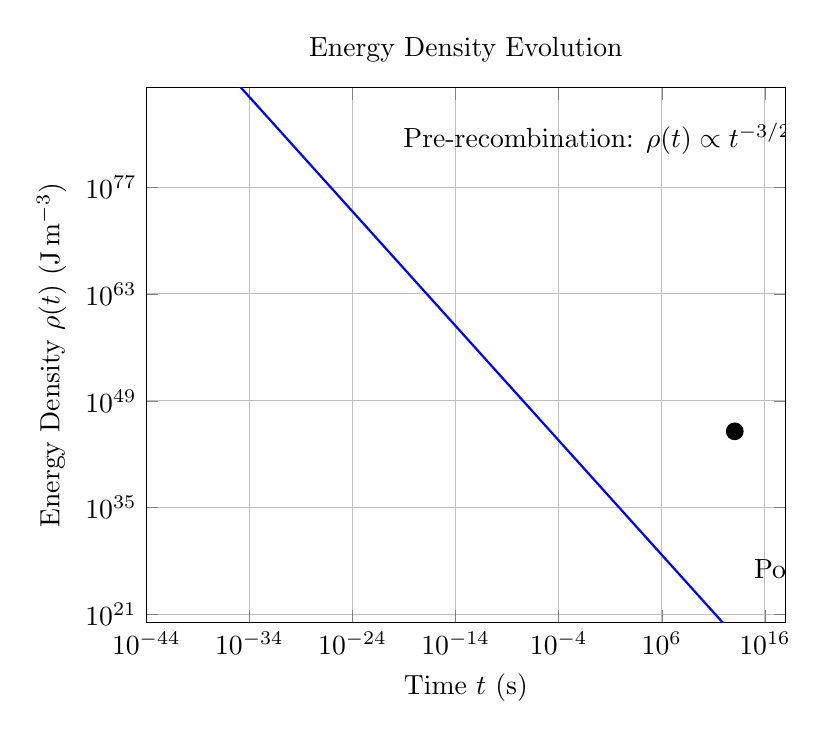
\begin{tikzpicture}
\begin{axis}[
    xlabel={Time $t$ (\si{\second})},
    ylabel={Energy Density $\rho(t)$ (\si{\joule\per\meter\cubed})},
    xmode=log,
    ymode=log,
    xmin=1e-44, xmax=1e18,
    ymin=1e20, ymax=1e90,
    grid=major,
    title={Energy Density Evolution},
    width=0.8\textwidth
]
\addplot[domain=1e-44:1.2e13, samples=100, blue, thick] {1e90*(x/1.616e-35)^(-1.5)};
\addplot[domain=1.2e13:1e18, samples=100, red, thick] {1e90*(1.2e13/1.616e-35)^(-1.5)*exp(-3*2.45e-17*(x-1.2e13)/2)};
\addplot[mark=*, only marks, mark size=3] coordinates {(1.2e13, 1e45)};
\node at (axis cs:1e-20,1e80) [anchor=south west] {Pre-recombination: $\rho(t) \propto t^{-3/2}$};
\node at (axis cs:1e14,1e30) [anchor=north west] {Post-recombination: $\rho(t) \propto e^{-3Ht}$};
\end{axis}
\end{tikzpicture}
\caption{Evolution of energy density $\rho(t)$, showing fractal scaling pre-recombination and exponential decay post-recombination at $t_{\text{rec}} = \SI{1.2e13}{\second}$.}
\label{fig:energy_density}
\end{figure}

\begin{figure}[h]
\centering
\begin{tikzpicture}
\begin{axis}[
    xlabel={Time $t$ (\si{\second})},
    ylabel={Horizon Radius $R(t)$ (\si{\meter})},
    xmode=linear,
    ymode=log,
    xmin=0, xmax=4.35e17,
    ymin=1e25, ymax=1e27,
    grid=major,
    title={Light Horizon Growth},
    width=0.8\textwidth
]
\addplot[domain=0:4.35e17, samples=100, green, thick] {1e26*exp(2.45e-17*x)};
\node at (axis cs:2e17,1e26.5) [anchor=north west] {$R(t) = R_0 e^{Ht}$};
\end{axis}
\end{tikzpicture}
\caption{Growth of the perceived light horizon radius $R(t)$, distinct from the fixed radius $R$ of $S^3$.}
\label{fig:horizon_growth}
\end{figure}

\section{Conclusions}
% Summarizing the model
The Fractal Bindu ($S^3$) model presents the Universe as a causally interdependent, compact three-dimensional sphere, where Bindu, as a \textit{skandha} and indestructible essence, unifies all scales through fractal phase transitions driven by the speed of light and the golden ratio. The light sphere creates the perceived expansion, with all phenomena arising within it. Existing outside time and existence, $S^3$ is the sole ontological foundation, supported by observational data, offering a complete framework for a continuous, interconnected reality.

\begin{thebibliography}{9}
\bibitem{Planck2018}
Planck Collaboration, ``Planck 2018 results. VI. Cosmological parameters,'' \textit{Astronomy \& Astrophysics}, vol. 641, A6, 2020.
\end{thebibliography}

\end{document}